\documentclass[conference]{IEEEtran}
\IEEEoverridecommandlockouts

\usepackage{cite}
\usepackage{amsmath,amssymb,amsfonts}
\usepackage{graphicx}
\usepackage{textcomp}
\usepackage{xcolor}
\usepackage{booktabs}
\usepackage{multirow}
\usepackage{array}
\usepackage{url}
\usepackage{placeins}
\setlength{\textfloatsep}{6pt plus 1pt minus 2pt}
\setlength{\floatsep}{6pt plus 1pt minus 2pt}
\setlength{\intextsep}{6pt plus 1pt minus 2pt}
\renewcommand{\topfraction}{0.95}
\renewcommand{\dbltopfraction}{0.95}
\renewcommand{\textfraction}{0.05}
\renewcommand{\floatpagefraction}{0.75}
\renewcommand{\dblfloatpagefraction}{0.75}

\def\BibTeX{{\rm B\kern-.05em{\sc i\kern-.025em b}\kern-.08em
    T\kern-.1667em\lower.7ex\hbox{E}\kern-.125emX}}

\begin{document}

\title{ORIGIN-Ax: Origin-Constrained Graph Refinement for Identifiable Latent Axes in Spatial Transcriptomics}

\author{\IEEEauthorblockN{Anonymous Authors}}

\maketitle
\begin{abstract}
Decomposition methods in spatial transcriptomics, such as NMF, ICA, and consensus factorization, convert high-dimensional tumor data into latent axes with gene loadings and spatial activity patterns. Yet in mixed tumor microenvironments, a coherent axis may reflect malignant biology, normal epithelium, stroma, immune infiltration, or unresolved mixtures rather than the intended target source. We present ORIGIN-Ax, a post-decomposition framework that recasts latent-axis interpretation as origin-constrained claim control. Given candidate axes from existing methods, ORIGIN-Ax constructs an origin-aware family graph, grouping axes only when expression loadings and cellular-source evidence are compatible. Families are labeled as target-supported, off-target, or non-identifiable using loading-weighted target evidence, off-target/decoy evidence, family consensus, held-out audits, and optional anchors. Across controlled benchmarks, pseudo-spatial mixtures, Xenium melanoma, target-swap controls, and a Visium HD colorectal cancer stress test, ORIGIN-Ax preserves recoverable target signals while reducing unsupported target-like promotions under predefined claim-risk audits. ORIGIN-Ax provides an auditable interpretation layer for gene-loading axes in complex spatial tissues.
\end{abstract}

\begin{IEEEkeywords}
spatial transcriptomics, latent-axis interpretation, gene programs, origin-constrained graph, claim control, tumor microenvironment
\end{IEEEkeywords}

\section{Introduction}

Spatial transcriptomics measures gene expression while preserving tissue location, enabling detailed studies of tumor architecture, immune infiltration, stromal remodeling, and spatially localized cell states~\cite{stahl2016visualization,tian2023expanding}. To summarize these high-dimensional measurements, many analyses apply decomposition methods such as non-negative matrix factorization (NMF), independent component analysis (ICA), or consensus factorization to extract latent expression programs~\cite{lee1999learning,hyvarinen2000ica,kotliar2019cnmf}. In this work, a \emph{latent axis} denotes a weighted gene program together with a spatial activity score across tissue locations.

However, the biological origin of such an axis is often ambiguous in tumor tissue. A spatially coherent factor enriched for plausible marker genes may not originate from the intended target cell population. Because malignant cells, normal epithelium, immune cells, stromal cells, and mixed boundary regions frequently occupy nearby spatial neighborhoods, a continuous expression axis may reflect target biology, off-target tissue structure, technical effects, or unresolved mixtures. The central difficulty is therefore not simply naming an axis, but determining whether a specific origin claim is sufficiently justified by the available evidence.

Existing evidence sources help but do not fully resolve this axis-level claim problem. Top genes, marker scores, and pathway enrichment describe program content~\cite{subramanian2005gsea,zhang2019cellmarker}; spatial maps show activity patterns; deconvolution estimates local cell-type composition~\cite{kleshchevnikov2022cell2location,cable2022rctd}; and orthogonal signals such as CNV inference, histology, or protein markers provide additional context. Nevertheless, these signals are rarely organized into a formal, transparent decision rule for whether a continuous gene-loading axis should be accepted as target-origin, rejected as off-target, or reported as non-identifiable. This gap often leads to subjective and difficult-to-audit interpretations across datasets and target definitions.

We formulate latent-axis interpretation as \emph{origin-constrained claim control}. Under this perspective, the key question is whether the evidence sufficiently supports the claim that an axis originates from a user-defined target source (e.g., malignant cells, myeloid inflammation, or stromal remodeling). A target claim should be promoted only when target evidence outweighs plausible competing origins; conversely, an axis should be rejected or labeled non-identifiable when normal epithelial, stromal, immune, endothelial, or technical decoy evidence provides a better explanation.

We introduce ORIGIN-Ax, a post-decomposition interpretation layer for gene-loading latent axes. ORIGIN-Ax does not replace upstream factorization methods but audits biological claims before downstream analysis. Given candidate axes, it constructs an origin-aware family graph whose edges depend on both expression similarity and origin evidence. Axes are grouped only when their loading patterns and source evidence are compatible, while seemingly similar axes better explained by different origins are deliberately separated. Thus, origin evidence actively shapes family structure rather than serving merely as a post-hoc score.

Each family receives a conservative label---target-supported, off-target, or non-identifiable---based on loading-weighted target evidence, off-target/decoy evidence, family consensus, held-out target-gene audits, and optional orthogonal anchors. Our contributions are threefold: (1) we recast latent-axis interpretation from marker-based annotation into origin-constrained claim control; (2) we introduce an origin-aware axis-family graph for evidence-driven grouping; and (3) we demonstrate, across controlled benchmarks, pseudo-spatial mixtures, real tumor datasets (Xenium melanoma and Visium HD colorectal cancer), and target-swap controls, that ORIGIN-Ax preserves recoverable target signals while reducing unsupported target-like promotions under predefined audit rules rather than estimating absolute biological false-positive rates.

\section{Related Work}

\subsection{Latent Decomposition and Gene Program Discovery}

NMF, ICA, and related factorization methods extract low-dimensional structure
from high-dimensional expression data~\cite{lee1999learning,hyvarinen2000ica}.
In single-cell and spatial transcriptomics, repeated or consensus-like
factorization and recent spatial co-expression module methods identify gene
programs, spatial factors, and activity gradients~\cite{kotliar2019cnmf,higgins2025stihc}.
These methods provide gene loadings and location-level scores, but they do not
by themselves decide whether a downstream target-origin claim is justified.
ORIGIN-Ax is complementary: it operates on candidate axes generated by upstream
methods and asks which axis-level biological claims are reliably supported.

\subsection{Annotation, Deconvolution, and External Evidence}

Standard interpretation tools include top-gene inspection, marker scoring,
pathway enrichment, and curated marker resources~\cite{subramanian2005gsea,zhang2019cellmarker}.
Spatial deconvolution estimates cell-type abundance in spots or
neighborhoods~\cite{kleshchevnikov2022cell2location,cable2022rctd}, and recent
spatial genomics discussions emphasize methods that connect spatial
measurements to explicit biological questions~\cite{jena2024openquestions}.
These evidence sources are useful, but they do not by themselves provide a
reproducible rule for whether a continuous gene-loading axis should be
interpreted as target-origin rather than off-target or mixed-origin signal.

\subsection{Origin-Aware Claim Control}

Most workflows ask whether a factor is stable, spatially coherent,
marker-enriched, or correlated with external covariates. ORIGIN-Ax instead
models competing origin evidence and performs interpretation at the family
level. A coherent family can be rejected when normal epithelial, stromal,
immune, endothelial, or technical evidence better explains the axis than the
target source. This distinguishes ORIGIN-Ax from expression-only clustering
followed by post-hoc annotation, because origin evidence actively shapes the
graph on which interpretable families are defined.

\section{Problem Formulation}

Let an upstream decomposition method, such as ICA, NMF, or
repeated NMF, produce a set of candidate latent axes
$\mathcal{A}=\{a_i\}_{i=1}^{m}$ from a spatial transcriptomic
expression matrix. Each axis $a_i=(\ell_i,z_i)$ contains a gene
loading vector $\ell_i$ and a spatial or neighborhood-level score
vector $z_i$. ORIGIN-Ax does not relearn the factorization of the
expression matrix. Instead, it addresses a post-decomposition
interpretation problem: given a user-defined target-origin claim,
determine whether the available evidence supports interpreting
one or more candidate axes as target-origin programs.

The inputs are candidate axes, target-support evidence, off-target or decoy
evidence representing plausible competing origins, and optional orthogonal
anchors such as cell-type labels, CNV-like latents, histology, or spatial niche
summaries. Held-out target genes, when available, are reserved for
post-refinement auditing rather than primary scoring. The output is a set of
refined axis families $\mathcal{F}=\{F_k\}$. The three semantic outcomes
correspond to target-supported, off-target, and non-identifiable claims, and are
reported using the implementation labels:
\[
\begin{aligned}
y(F_k)\in\{&
\texttt{target\_axis},\texttt{off\_target},\\
&\texttt{non\_identifiable}\}.
\end{aligned}
\]
A separate output flag \texttt{not\_target\_axis} is used only to exclude
families from target-origin downstream analyses; it is not a fourth semantic
category.

This formulation is claim-control oriented. The goal is not to
assign every latent axis the most plausible biological name, nor to
force every stable factor into a target category. Instead, ORIGIN-Ax
asks whether a specific target-origin interpretation is sufficiently
supported relative to predefined competing origins. A family is
promoted only when target evidence outweighs competing evidence
under fixed decision rules and the family is internally consistent;
it is rejected when an off-target origin better explains the axis;
and it is marked non-identifiable when the available candidates,
references, or anchors are insufficient to support a safe
target-origin claim.

\section{Methods}

\begin{figure*}[!t]
\centering
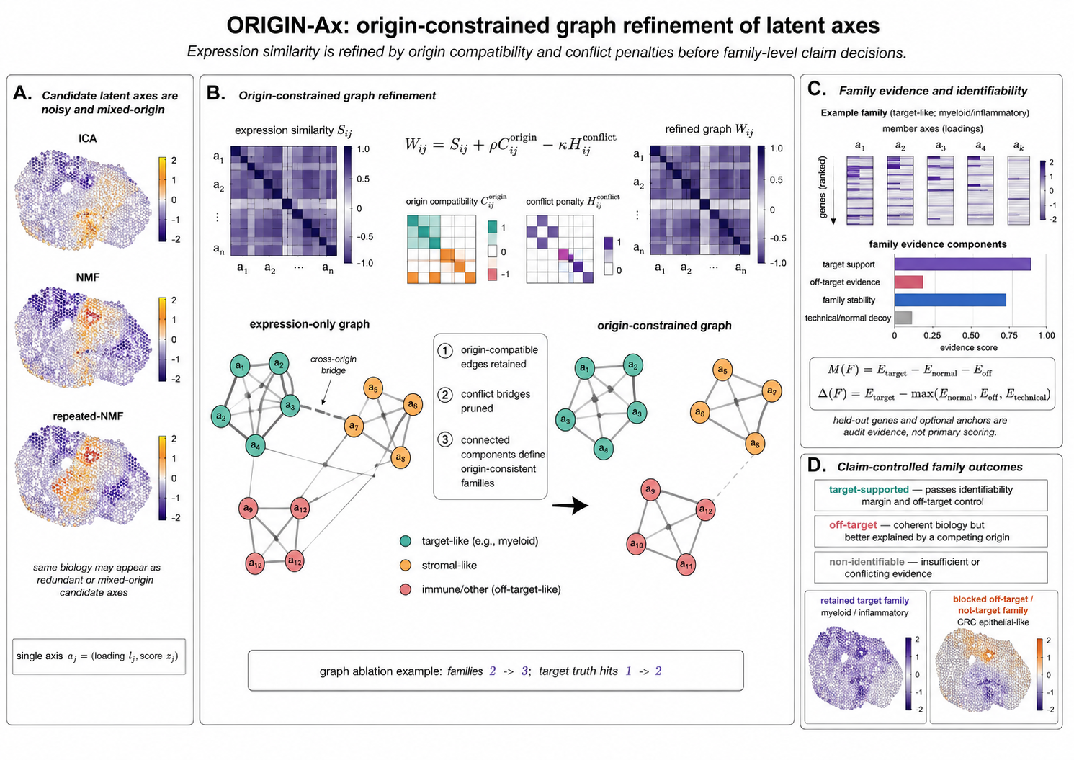
\includegraphics[width=0.94\linewidth]{figures/fig1_workflow.pdf}
\caption{ORIGIN-Ax converts candidate axes into origin profiles, refines them
with compatibility- and conflict-aware graph edges, assembles origin-consistent
families, and assigns target-supported, off-target, or non-identifiable labels.}
\label{fig:workflow}
\end{figure*}

\subsection{Overview}

Given the claim-control problem defined above, ORIGIN-Ax implements a
post-decomposition refinement layer over candidate latent axes
(Fig.~\ref{fig:workflow}). The method proceeds in four steps. First, it
computes expression similarity and competing-origin profiles for candidate
axes. Second, it builds an origin-constrained axis graph in which edges are
strengthened by compatible origin evidence and weakened by cross-origin
conflict. Third, connected components of this graph define axis families,
whose loadings and scores are direction-aligned to form family consensus
axes. Finally, each family is assigned a claim label using target support,
competing off-target evidence, family stability, held-out audits, and
optional orthogonal anchors.

The upstream method provides candidate loadings and spatial scores, whereas
ORIGIN-Ax controls which target-origin claims are allowed downstream. Outputs
include member axes, consensus loadings, evidence components, graph diagnostics,
claim labels, and rationales.

\subsection{Candidate Axis Interface}

ORIGIN-Ax assumes candidate axes already exist. In our experiments, axes are
obtained from raw ICA, raw NMF, high-target subset decompositions, or
repeated-NMF runs. Each axis must provide a gene loading vector and a spatial or
neighborhood-level score vector; no reconstruction objective is re-optimized.
This minimal interface lets ORIGIN-Ax refine ICA-only, NMF-only, or repeated-NMF
outputs with the same graph, scoring, and labeling rules.

\subsection{Origin-Constrained Axis Family Graph}

Candidate axes are grouped before interpretation, but family construction is
not based on expression similarity alone. For axes $a_i$ and $a_j$, ORIGIN-Ax
first computes an expression similarity
\begin{equation}
S(a_i,a_j)=0.6|\mathrm{corr}(\ell_i,\ell_j)|+0.4J(T_i,T_j),
\end{equation}
where $T_i$ is the top-gene set of axis $a_i$ and $J(\cdot,\cdot)$ is Jaccard
similarity. Loading correlation captures global agreement across genes,
whereas top-gene overlap captures whether the interpretable high-loading tail
is shared.

Each axis also receives a competing-origin profile
\begin{equation}
e_i=(E_{\mathrm{target},i},E_{\mathrm{normal},i},
E_{\mathrm{TME},i},E_{\mathrm{tech},i}),
\end{equation}
where each term is computed from loading-tail-weighted gene evidence using
the positive high-loading genes of $a_i$. The dominant origin is the largest
entry of $e_i$, and the axis margin is
\[
\delta_i=E_{\mathrm{target},i}
-\max(E_{\mathrm{normal},i},E_{\mathrm{TME},i},E_{\mathrm{tech},i}).
\]

ORIGIN-Ax then refines the edge weight as
\begin{equation}
W_{ij}=S(a_i,a_j)+\rho C^{\mathrm{origin}}_{ij}
-\kappa H^{\mathrm{conflict}}_{ij},
\end{equation}
where $C^{\mathrm{origin}}_{ij}\in[0,1]$ is the cosine similarity between
origin profiles when the dominant origin agrees and is set to zero otherwise.
$H^{\mathrm{conflict}}_{ij}\in[0,1]$ is set to one for strong cross-origin
bridge edges, including target-dominant versus off-target-dominant pairs with
sufficient evidence. Otherwise, it combines target/off-target co-activation,
margin sign flips, and dominant-origin disagreement.

Thus, origin-compatible axes are more likely to remain connected, while
expression-similar axes with competing origins are pruned. In our experiments,
$\rho=0.15$, $\kappa=0.60$, and edges are retained when $W_{ij}\geq0.35$.
These constants are not treated as dataset-specific optima. We use fixed
defaults to avoid post-hoc tuning on the evaluation datasets; their role is to
define a transparent audit rule in which conflict pruning dominates
compatibility reward. We therefore report score-threshold, graph-threshold, and
ablation audits rather than learning separate hyperparameters per dataset.

Connected components of the origin-constrained graph define axis families.
Member loadings are direction-aligned before computing a consensus loading and
score. The consensus is the aligned average of benchmark-provided axes, not a
new factor learned by re-optimizing the expression matrix. Each final family is
traceable to its member axes, source methods, pairwise similarities,
compatibility terms, and conflict penalties.

\subsection{Origin Evidence Vector}

For each gene $g$, a target definition provides target support $u_g$, normal
or target-specific penalty $r_g$, and off-target penalty $o_g$. For a family
$F$, ORIGIN-Ax computes loading-tail-weighted evidence over the positive
high-loading genes:
\begin{equation}
E_{\mathrm{target}}(F)=
\frac{\sum_{g\in P_F}w_{Fg}u_g}
{\sum_{g\in P_F}w_{Fg}+\epsilon},
\end{equation}
\begin{equation}
E_{\mathrm{normal}}(F)=
\frac{\sum_{g\in P_F}w_{Fg}r_g}
{\sum_{g\in P_F}w_{Fg}+\epsilon},
\end{equation}
\begin{equation}
E_{\mathrm{off}}(F)=
\frac{\sum_{g\in P_F}w_{Fg}o_g}
{\sum_{g\in P_F}w_{Fg}+\epsilon}.
\end{equation}
Here $P_F$ is the positive top-loading tail of the consensus axis and $w_{Fg}$
is the positive loading weight. The target-origin margin is
\[
M(F)=E_{\mathrm{target}}(F)-E_{\mathrm{normal}}(F)-E_{\mathrm{off}}(F),
\]
and the identifiability margin is
\begin{equation}
\begin{split}
\Delta(F)=&\,E_{\mathrm{target}}(F)\\
&-\max(E_{\mathrm{normal}}(F),E_{\mathrm{off}}(F),
E_{\mathrm{technical}}(F)).
\end{split}
\end{equation}

Family stability is
\begin{equation}
Q(F)=0.4\min(1,|F|/4)+0.3\min(1,d_F/3)+0.3\bar{s}_F,
\end{equation}
where $|F|$ is member count, $d_F$ is the number of contributing decomposition
sources, and $\bar{s}_F$ is mean within-family loading similarity.

Target and off-target definitions are supplied as binary or confidence-weighted
references rather than learned from the test set. Target support may come from
malignant-only references, high-CNV regions, or curated programs; off-target
references cover normal epithelial, stromal, immune, endothelial, and
tissue-specific false-boundary programs. Anchor genes are removed from
off-target sets in anchor-split experiments, while overlapping non-anchor
markers remain competing evidence. Technical evidence is reserved for supplied
technical references or covariates. CRC gene weights were derived from
CellMarker~\cite{zhang2019cellmarker} and curated false-boundary programs;
Xenium melanoma references were pre-specified marker sets. In target-swap,
stromal/ECM genes become the target and myeloid genes become off-target.

\subsection{Scoring, Auditing, and Labels}

ORIGIN-Ax uses percentile-normalized evidence values:
\begin{equation}
\mathrm{score}(F)=0.6\widetilde{M}(F)+0.4\widetilde{Q}(F)
-\widetilde{E}_{\mathrm{off}}(F).
\end{equation}
Percentile normalization uses the 5th--95th percentile range across families
within the same run. The three terms have distinct roles: target margin
promotes origin support, family stability prevents single-axis
overinterpretation, and off-target affinity implements negative evidence.

The fixed label rules are as follows. A family is labeled \texttt{target\_axis}
if $\mathrm{score}(F)>0.2$, $\Delta(F)>0$, and mean family-origin conflict is
at most 0.35. A family is labeled \texttt{off\_target} if
$\mathrm{score}(F)<-0.2$, $\Delta(F)<-0.05$, or target-specific off-target
evidence dominates. Remaining families are labeled
\texttt{non\_identifiable}. Thus, the output label space controls claims:
\texttt{target\_axis} supports target-origin interpretation,
\texttt{off\_target} denotes coherent non-target biology,
\texttt{non\_identifiable} marks insufficient or mixed evidence.
\texttt{not\_target\_axis} is an implementation flag used to exclude a family
from target-origin claims; it is not a fourth semantic label.

A target-specific off-target override is triggered when top genes contain at
least two markers from a pre-specified forbidden source, such as stromal/ECM,
endothelial, normal epithelial, or malignant-melanoma decoys under a myeloid
target definition. Optional anchors support attribution checks but cannot rescue
a family whose gene-origin evidence fails. To reduce circularity, positive
experiments split target genes into anchor and held-out subsets; only anchors
contribute to primary scoring, while held-out genes audit strict positives. The
method is rule-based rather than a trained classifier because labeled target and
false-target axes across tissues, platforms, and target definitions are not
available at sufficient scale.

\subsection{Implementation and Reproducibility}

All experiments use fixed seeds and write candidate-axis tables, origin-graph
edge audits, family tables, score diagnostics, and final claim summaries. An
automated check verifies the real-positive strict family, forbidden off-target
rejection, CRC Axis-5-like non-promotion, positive recovery, benchmark
refinement, and target-swap behavior.

\subsection{Computational Complexity}

ORIGIN-Ax is applied after decomposition, so its scaling is dominated by the
number of candidate axes rather than the number of spatial bins. For $m$
candidate axes and $p$ genes, pairwise graph construction costs $O(m^2p)$ for
loading similarity plus top-gene overlap, family scoring costs $O(|F|p)$ for
each family $F$, and the similarity matrix requires $O(m^2)$ memory. In our
benchmark-refinement runs, $m$ is 10--32; even for 500 candidate axes, the dense
float64 similarity matrix is approximately 2 MB, although pairwise loading
comparisons become the dominant step. Thus the computational overhead is small
relative to upstream factorization on the candidate pools evaluated here. For
atlas-scale candidate pools with hundreds to thousands of axes, the quadratic
term can dominate; practical implementations can restrict pairwise comparisons
to top-neighbor loading matches or block candidates by upstream method and seed,
but such acceleration was not evaluated in this study.

\section{Experiments}

\subsection{Datasets and Benchmark Inputs}

We evaluate ORIGIN-Ax in controlled positives with planted target/off-target
blocks, semi-real pseudo-spatial mixtures from Xenium melanoma cells, real
Xenium melanoma neighborhoods with a myeloid/inflammatory target, a
myeloid-to-stromal target-swap control, and a sampled Visium HD CRC stress test
for epithelial overcalling. To test decomposition-agnostic refinement, ORIGIN-Ax
is applied to raw ICA-only, NMF-only, and repeated-NMF consensus-like candidate
axes without regenerating mixed candidates.

\subsection{Evaluation Metrics}

For positives, we report target recovery, held-out target-gene overlap, and, in
real positives, strict positives: target-supported families with held-out
overlap and no forbidden off-target source. For stress tests, we report
unsupported target-like promotions before and after refinement. These are
predefined claim-risk audit events rather than ground-truth false-positive
labels. A candidate is counted as unsupported when it satisfies naive
target-like criteria but lacks held-out support, is dominated by decoy evidence,
or fails the identifiability margin under the specified reference universe. For
CRC, where true malignant-axis labels are unavailable, this means quantifying
malignant-like promotion risk under epithelial-marker, CNV-association, and
high-CNV-presence rules, not claiming absolute biological false positives.

\subsection{Ablation Protocol}

To evaluate whether each evidence component contributes to refinement, we add
fixed ablations using the same candidate axes and family tables. The ablations
do not tune thresholds or regenerate candidates. We compare the full model
against: (i) candidate-level interpretation without family refinement, (ii)
removal of the off-target penalty, and (iii) removal of the stability term. We
additionally compare expression-only graph construction against
origin-constrained graph construction on the controlled positive.

For parameter calibration, controlled and pseudo-ST settings serve as
development audits. We scan $\rho\in\{0,0.05,0.10,0.15,0.20,0.30\}$,
$\kappa\in\{0.20,0.40,0.60,0.80,1.00\}$, edge thresholds
$\{0.25,0.30,0.35,0.40,0.45\}$, target/stability weights
$\{0.50/0.50,0.60/0.40,0.70/0.30\}$, and score thresholds
$\{0.10,0.15,0.20,0.25,0.30\}$. A graph tuple is stable if the family count differs
from the selected default by at most one, removes cross-origin bridge edges, and
does not reduce downstream recovery in every development setting; a score tuple
is stable if it retains at least one truth-supported family and produces no
unsupported target call. We also compare top-marker and target-only
interpretation baselines, compute random gene-set margin nulls, and report
reference-coverage warnings before biological interpretation. Reference warnings
are issued for off-target coverage below 0.30, decoy diversity below 2,
ambiguous-marker fraction above 0.25, or top-gene reference hit rate below 0.15.
To test reference-deletion robustness, we additionally removed 20\%, 40\%, and
60\% of off-target reference genes in the real-positive Xenium setting and
tracked strict-target retention and forbidden off-target rejection.

\section{Results}

\subsection{ORIGIN-Ax Retains Target Recovery While Reducing Unsupported Calls}

Across controlled and semi-real positives, ORIGIN-Ax recovered target-origin
families (Fig.~\ref{fig:evidence}). In the controlled positive, it recovered
two target families from 40 candidates and 3 families; balanced and low-purity
pseudo-ST recovered one target family each. In benchmark-refinement mode,
ORIGIN-Ax retained truth-supported pseudo-ST recovery across ICA, NMF, and
repeated-NMF consensus-like inputs while reducing unsupported target-like
promotions under the predefined audit rules (Table~\ref{tab:benchmark}). This
supports the intended role of ORIGIN-Ax as a refinement layer: it reduces
candidate-level overpromotion without replacing upstream decomposition.

\begin{figure}[!t]
\centering
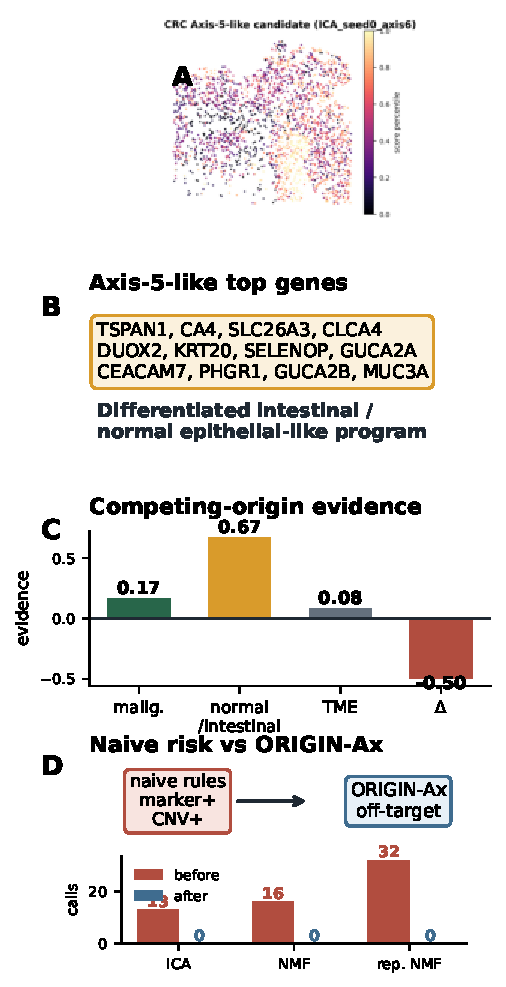
\includegraphics[width=\linewidth]{figures/fig4_crc_axis5_singlecol.pdf}
\caption{CRC epithelial-like stress test. (A) Axis-5-like spatial score map.
(B) Differentiated intestinal / normal epithelial top genes. (C) Normal decoy
evidence gives a negative identifiability margin. (D) ORIGIN-Ax blocks
malignant-like promotion risk across ICA, NMF, and repeated-NMF inputs.}
\label{fig:crc}
\end{figure}

\begin{figure}[!t]
\centering
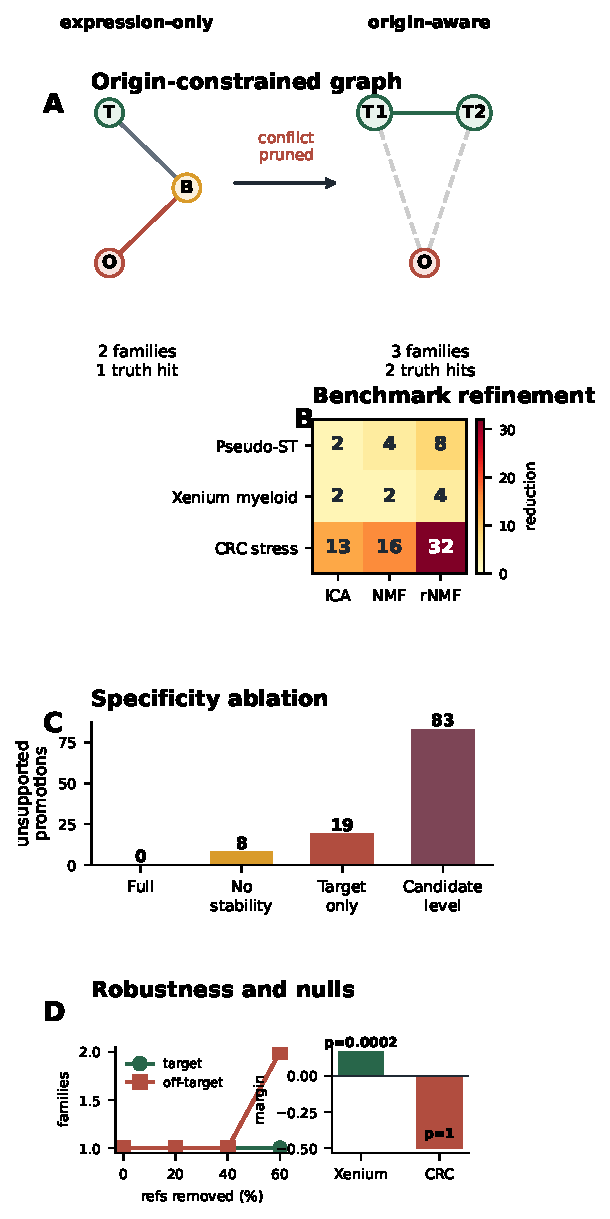
\includegraphics[width=\linewidth]{figures/fig2_evidence_summary_singlecol.pdf}
\caption{Ablation and audit evidence. (A) Origin-constrained graph refinement
changes family construction. (B) Unsupported target-like promotions are reduced
across inputs. (C) Off-target evidence and family refinement drive specificity.
(D) Reference-deletion and random gene-set null audits support the real-positive
target family and reject the CRC Axis-5-like program.}
\label{fig:evidence}
\end{figure}

\begin{table*}[t]
\caption{Benchmark-refinement results. ``Before'' counts unsupported
target-like calls from benchmark axes; ``After'' counts unsupported calls after
ORIGIN-Ax refinement. CRC entries are claim-risk audits, not ground-truth
false-positive rates.}
\label{tab:benchmark}
\centering
\scriptsize
\setlength{\tabcolsep}{3pt}
\begin{tabular}{p{0.15\linewidth}p{0.15\linewidth}rrrrrp{0.24\linewidth}}
\toprule
Dataset & Input & Axes & Fam. & Before & After & Target & Conclusion \\
\midrule
Pseudo-ST & raw ICA & 10 & 4 & 2 & 0 & 2 & Truth retained \\
Pseudo-ST & NMF & 10 & 5 & 4 & 0 & 2 & Truth retained \\
Pseudo-ST & rep. NMF & 20 & 5 & 8 & 0 & 2 & Truth retained \\
Xenium & raw ICA & 12 & 3 & 2 & 0 & 0 & Off-target rejected; target absent \\
Xenium & NMF & 12 & 4 & 2 & 0 & 1 & Strict positive; off-target rejected \\
Xenium & rep. NMF & 24 & 4 & 4 & 0 & 1 & Strict positive; off-target rejected \\
CRC & raw ICA & 16 & 6 & 13 & 0 & 0 & Off-target families rejected \\
CRC & NMF & 16 & 5 & 16 & 0 & 0 & Axis-5-like rejected \\
CRC & rep. NMF & 32 & 5 & 32 & 0 & 0 & Axis-5-like rejected \\
\bottomrule
\end{tabular}
\setlength{\tabcolsep}{6pt}
\end{table*}

\begin{table}[!t]
\caption{Interpretation-layer baseline audit aggregated across benchmark rows.}
\label{tab:interpretation_baselines}
\centering
\scriptsize
\setlength{\tabcolsep}{3pt}
\begin{tabular}{p{0.46\linewidth}rrr}
\toprule
Interpretation rule & Target & Unsupported & Truth \\
\midrule
Candidate-level top-gene style & 118 & 83 & 39 \\
Target evidence only & 33 & 19 & 15 \\
No family stability & 17 & 8 & 10 \\
ORIGIN-Ax full & 7 & 0 & 7 \\
\bottomrule
\end{tabular}
\setlength{\tabcolsep}{6pt}
\end{table}

\begin{table}[!t]
\caption{Compact calibration, baseline, reference, and scaling audits.}
\label{tab:robustness}
\centering
\scriptsize
\setlength{\tabcolsep}{2pt}
\begin{tabular}{p{0.31\linewidth}p{0.63\linewidth}}
\toprule
Audit & Result \\
\midrule
Parameter calibration &
Graph defaults are in the stable plateau: 47/150 tuples stable; score decisions
were robust across all 15 tested tuples on controlled and pseudo-ST settings. \\
Interpretation baselines &
Unsupported promotions: top-marker 83, target-only 19, no-stability 8,
ORIGIN-Ax full 0. \\
Reference coverage &
Four target settings triggered no coverage warning; off-target coverage was
0.77--1.00 and decoy diversity was 2--9. \\
Null margins and scaling &
Xenium F0 margin $p=2.0{\times}10^{-4}$; CRC Axis-5 malignant margin $p=1.0$.
At 1000 axes, the pairwise matrix is 8.0 MB but graph construction remains
$O(m^2p)$. \\
\bottomrule
\end{tabular}
\setlength{\tabcolsep}{6pt}
\end{table}

\subsection{Real Xenium Melanoma: Target and Off-Target Refinement}

In real Xenium melanoma neighborhoods, ORIGIN-Ax identified F0 as a strict
myeloid/inflammatory target family with held-out target-gene overlap of 4, no
dominant forbidden off-target source, and a significant random gene-set margin
audit ($p=2.0\times 10^{-4}$). In the same experiment, F1 contained malignant
melanoma markers including \textit{TYRP1}, \textit{PMEL}, \textit{TYR}, and
\textit{MLANA}; ORIGIN-Ax labeled it malignant-melanoma-like and set the
\texttt{not\_target\_axis} filtering flag. F0 and F1 therefore show acceptance
and rejection under the same evidence rules.

\subsection{Target-Swap Demonstrates Target-Agnostic Refinement}

Using the same Xenium candidate axes, we changed the target definition from
myeloid/inflammatory to stromal/fibroblast/ECM. The myeloid-like family was not
a stromal target, whereas the stromal F2-like family was rejected under the
myeloid target but recovered as \texttt{target\_axis} under the stromal target
(Fig.~\ref{fig:swap}). Thus ORIGIN-Ax is target-definition aware rather than a
fixed marker filter.

\begin{figure}[!t]
\centering
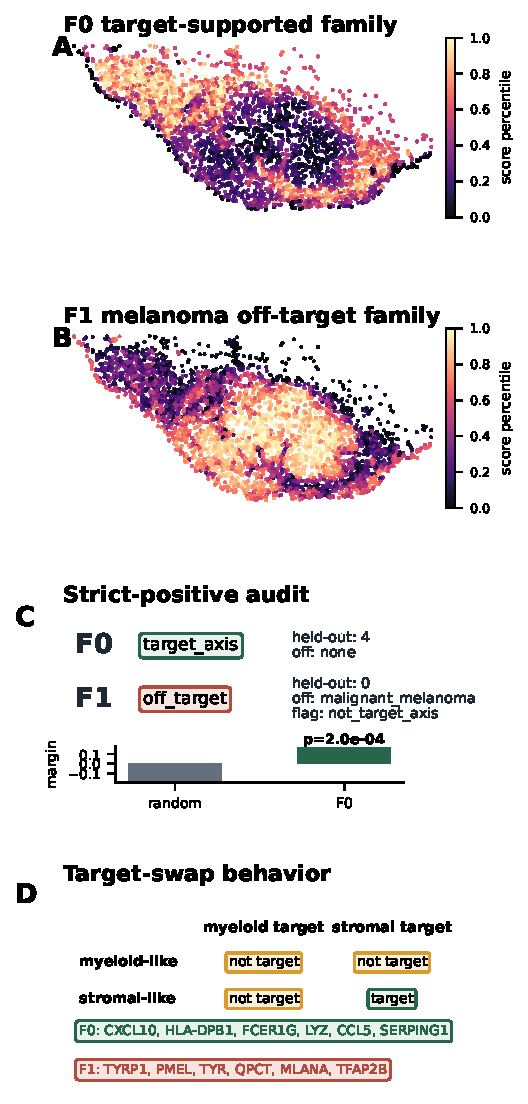
\includegraphics[width=\linewidth]{figures/fig3_target_swap_singlecol.pdf}
\caption{Real Xenium target refinement and target-swap behavior. (A) Myeloid
target family. (B) Stromal off-target family. (C) Strict-positive and
off-target calls. (D) The same families change calls when the target definition
is swapped.}
\label{fig:swap}
\end{figure}

\subsection{Ablation and Sensitivity Audits}

The audit supports origin-constrained graph construction, off-target rejection,
and family refinement (Fig.~\ref{fig:evidence}C). In the controlled positive,
the expression-only graph produced 2 families, whereas the origin-constrained
graph produced 3 families and removed cross-origin bridge edges; target truth
hits increased from 1 to 2 without adding false target calls. Aggregated
baselines show the interpretation-layer effect: candidate-level top-gene style
promotion yields 83 unsupported promotions, target evidence alone yields 19,
removing family stability yields 8, and full ORIGIN-Ax keeps 7 truth-supported
calls without unsupported promotions (Table~\ref{tab:interpretation_baselines}).
Additional audits place the fixed graph and score defaults inside stable
development-set plateaus, show no reference-coverage warnings across four target
settings, and support the Xenium target margin but not the CRC Axis-5-like
malignant margin (Table~\ref{tab:robustness}).
Reference deletion retained one strict myeloid target family and at least one
forbidden off-target rejection across 20\%--60\% deletion.

\subsection{Visium HD CRC: Blocking Promotion When Decoy Evidence Dominates}

In the Visium HD CRC stress test, an Axis-5-like program contained
differentiated intestinal and normal epithelial genes including \textit{TSPAN1},
\textit{CA4}, \textit{SLC26A3}, \textit{CLCA4}, \textit{KRT20}, and
\textit{CEACAM7}. Naive epithelial-marker, CNV-association, and high-CNV
presence rules would call this program malignant-like. ORIGIN-Ax instead
labeled it \texttt{normal\_epithelial\_like}/off-target, with zero CRC target
calls after target-specific off-target refinement across ICA, NMF, and
repeated-NMF inputs. This blocks a concrete overinterpretation path when
target-origin evidence is inadequate.

\section{Discussion and Limitations}

ORIGIN-Ax provides an auditable evidence framework for latent-axis
interpretation. Across experiments, target recovery is retained in positives,
unsupported target-like calls are reduced in benchmark-refinement audits, a
forbidden off-target family is rejected in real Xenium melanoma, a stromal
family becomes target only under a stromal target definition, and a CRC
epithelial program is not overcalled as malignant.

In practice, a user runs ICA, NMF, repeated-NMF consensus-like analysis, or
another decomposition, then ORIGIN-Ax uses loadings, scores, target support,
off-target references, and optional anchors to produce family tables,
strict-positive summaries, off-target warnings, and claim recommendations.
References should be defined before final calling, include plausible
false-boundary programs, and split target genes into anchor and held-out subsets
when possible. ORIGIN-Ax uses transparent rule-based evidence integration rather
than a trained classifier because labeled target and false-target axes across
tissues, platforms, and target definitions are not available at sufficient
scale.

For reproducibility, ORIGIN-Ax is structured as a scriptable Python workflow:
candidate-axis tables, reference gene weights, family graphs, score tables,
strict-positive audits, robustness summaries, and plotting inputs are written as
plain CSV files. The anonymous review repository is available at
\url{https://anonymous.4open.science/r/ORIGIN-Ax}. It includes code, fixed
seeds, reference sets, processed result tables, and figure-generation scripts so
that users can rerun the refinement layer on their own ICA, NMF, or repeated-NMF
candidate axes.

ORIGIN-Ax provides claim control under available evidence rather than solving
all mixture and origin-identification problems in spatial tumor data. Its
decisions are conditional on the user-defined reference universe: an undefined
decoy origin cannot be rejected, and incomplete off-target references can
convert a false boundary into an apparent target-supported call. Overlapping
markers are treated as competing evidence rather than automatically assigned to
the target, but the result remains conditional on reference quality and
coverage. It does not
perform expression decontamination, infer ground-truth cell-of-origin, prove
clone/niche causality, or replace wet-lab validation. ORIGIN-Ax also cannot
recover a target program that the upstream decomposition never exposed; absence
of a target call may reflect candidate-generation failure rather than biological
absence. Non-identifiable is therefore a valid algorithm output, indicating that
the current candidates, references, and anchors are insufficient to safely
support a biological claim. Thresholds are fixed and reported here, and
sensitivity audits expose how score and family thresholds affect calls. Future
work can add additional evidence sources and uncertainty estimates, but the
present contribution is a post-decomposition origin-constrained graph refinement
layer.

\section{Conclusion}

ORIGIN-Ax is a decomposition-agnostic origin-constrained graph refinement
framework for latent axes in complex spatial transcriptomics data. By combining
expression similarity, origin compatibility, off-target conflict, axis-family
consensus, and non-identifiability labels, it turns candidate gene programs into
auditable target-origin claims. In our audits, this preserves supported target
families, rejects off-target families, and clarifies when an attractive axis
should remain non-identifiable. The framework does not replace upstream
decomposition or prove cell-of-origin, but it provides a practical layer for
preserving supported axes while blocking unsupported biological overpromotion.

\FloatBarrier
\section*{Acknowledgment}

Omitted for anonymous review.

\bibliographystyle{IEEEtran}
\bibliography{references}

\end{document}
